\begin{figure}[h]
	\centering
	\setlength{\resLen}{0.85in}
	\addtolength{\tabcolsep}{-4pt}
	\begin{tabular}{ccccccc}
		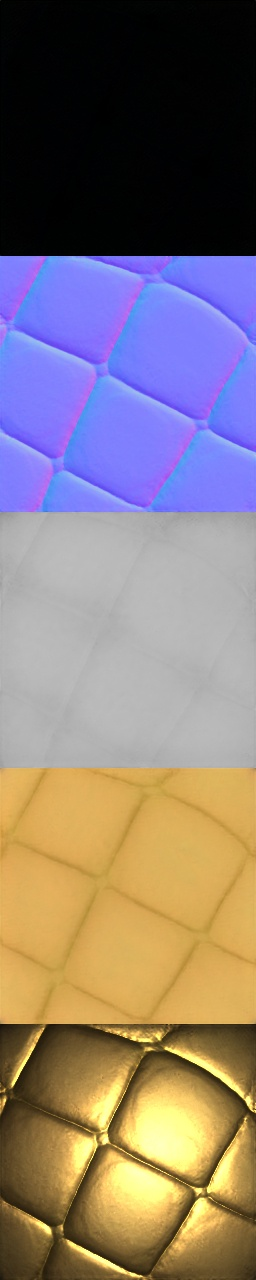
\includegraphics[width=\resLen]{svbrdf/others/matgan/04.jpg} &
		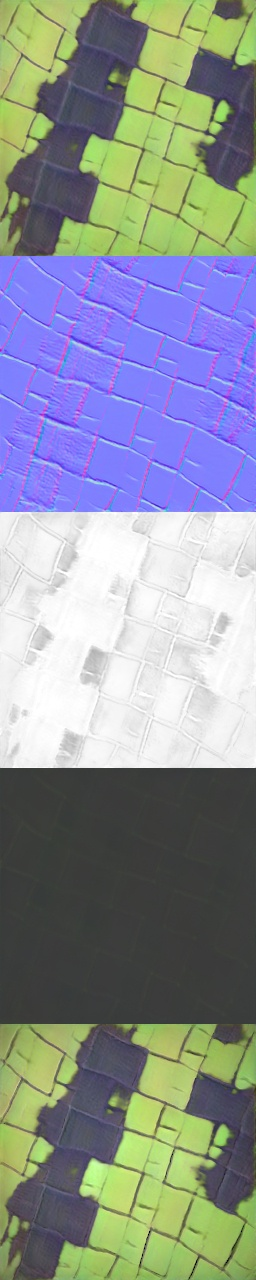
\includegraphics[width=\resLen]{svbrdf/others/matgan/05.jpg} &
		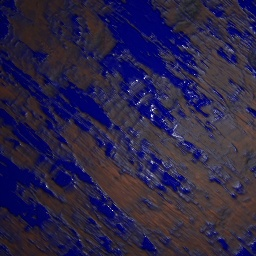
\includegraphics[width=\resLen]{svbrdf/others/matgan/08.jpg} &
		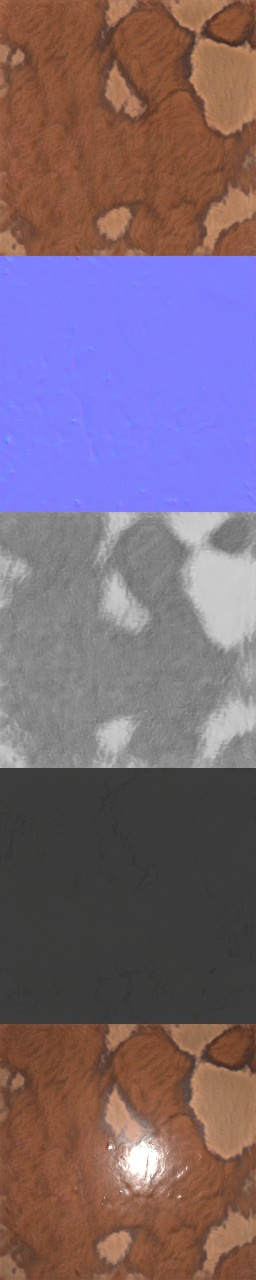
\includegraphics[width=\resLen]{svbrdf/others/matgan/10.jpg} &
		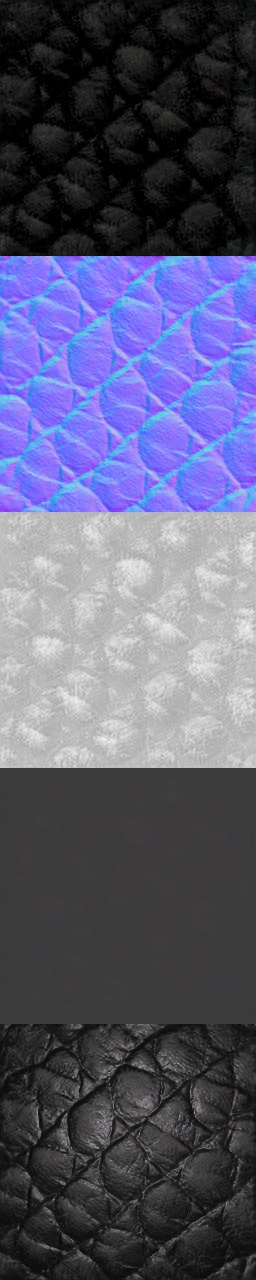
\includegraphics[width=\resLen]{svbrdf/others/matgan/11.jpg} &
		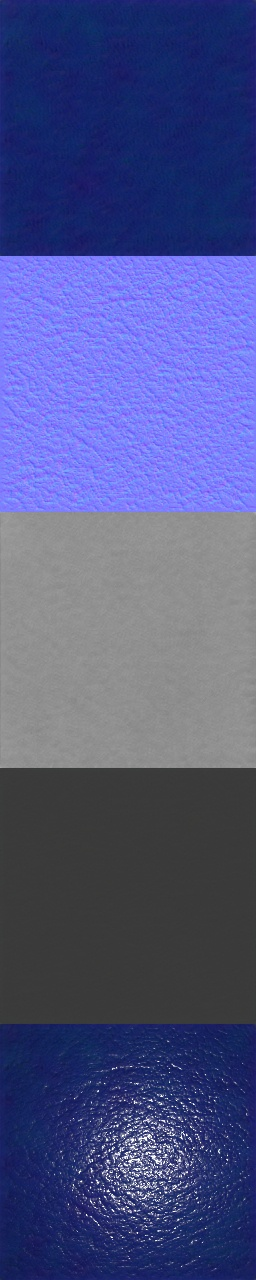
\includegraphics[width=\resLen]{svbrdf/others/matgan/12.jpg} &
		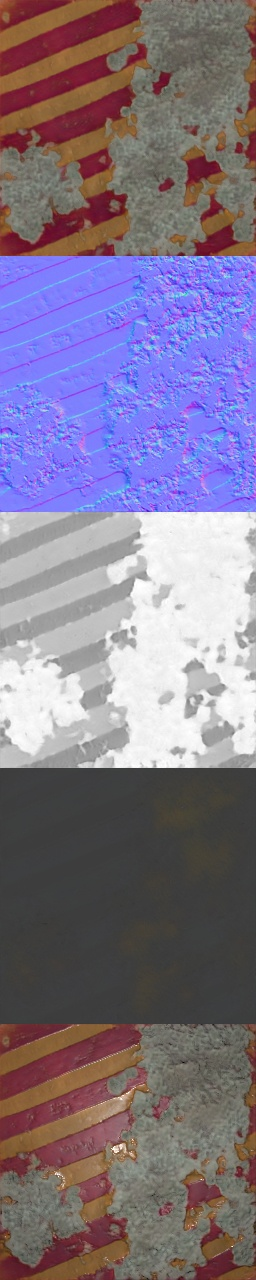
\includegraphics[width=\resLen]{svbrdf/others/matgan/19.jpg}
	\end{tabular}
	\caption[Materials generated by MaterialGAN]{\label{fig:svbrdf:matgan}
		\textbf{Seven materials generated by randomly sampling MaterialGAN.} Top to bottom: diffuse albedo, normal, roughness, specular albedo and renderings under flash illumination. As can be seen, the material maps are high-quality with meaningful correlations both spatially and across materials parameters, and visually look like plausible real-world materials.
	}
\end{figure}